%% Template para dissertação/tese na classe UFPEthesis
%% versão 0.9.2
%% (c) 2005 Paulo G. S. Fonseca
%% www.cin.ufpe.br/~paguso/ufpethesis

%% Carrega a classe ufpethesis
%% Opções: * Idiomas
%%           pt   - português (padrão)
%%           en   - inglês
%%         * Tipo do Texto
%%           bsc  - para monografias de graduação
%%           msc  - para dissertações de mestrado (padrão)
%%           qual - exame de qualificação doutorado
%%           prop - proposta de tese doutorado
%%           phd  - para teses de doutorado
%%         * Mídia
%%           scr  - para versão eletrônica (PDF) / consulte o guia do usuario
%%         * Estilo
%%           classic - estilo original à la TAOCP (deprecated)
%%           std     - novo estilo à la CUP (padrão)
%%         * Paginação
%%           oneside - para impressão em face única
%%           twoside - para impressão em frente e verso (padrão)
\documentclass[bsc, oneside]{UFPEThesis/ufpethesis}

%% Preâmbulo:
%% coloque aqui o seu preâmbulo LaTeX, i.e., declaração de pacotes,
%% (re)definições de macros, medidas, etc.

%% Identificação:

% Universidade
% e.g. \university{Universidade de Campinas}
% Na UFPE, comente a linha a seguir
\university{Universidade Federal de Pernambuco}

% Endereço (cidade)
% e.g. \address{Campinas}
% Na UFPE, comente a linha a seguir
% \address{<CIDADE DA IES>}

% Instituto ou Centro Acadêmico
% e.g. \institute{Centro de Ciências Exatas e da Natureza}
% Comente se não se aplicar
\institute{Centro de Informática}

% Departamento acadêmico
% e.g. \department{Departamento de Informática}
% Comente se não se aplicar
% \department{<NOME DO DEPARTAMENTO>}

% Programa de pós-graduação
% e.g. \program{Pós-graduação em Ciência da Computação}
\program{Bacharelado em Ciência da Computação}

% Área de titulação
% e.g. \majorfield{Ciência da Computação}
\majorfield{Ciência da Computação}

% Título da dissertação/tese
% e.g. \title{Sobre a conjectura $P=NP$}
\title{Previsão imediata de sequências de sinais de áudio como método de redução de latência em transmissões online}

% Data da defesa
% e.g. \date{19 de fevereiro de 2003}
% \date{<DATA DA DEFESA>}

% Autor
% e.g. \author{José da Silva}
\author{Luiz Henrique Tavares Caúla}

% Orientador(a)
% Opção: [f] - para orientador do sexo feminino
% e.g. \adviser[f]{Profa. Dra. Maria Santos}
\adviser{Filipe Carlos de Albuquerque Calegario}

% Orientador(a)
% Opção: [f] - para orientador do sexo feminino
% e.g. \coadviser{Prof. Dr. Pedro Pedreira}
% Comente se não se aplicar
% \coadviser{NOME DO(DA) CO-ORIENTADOR(A)}

%% Inicio do documento
\begin{document}

%%
%% Parte pré-textual
%%
\frontmatter

% Folha de rosto
% Comente para ocultar
\frontpage

% Portada (apresentação)
% Comente para ocultar
\presentationpage

% Dedicatória
% Comente para ocultar
% \begin{dedicatory}
% <DIGITE A DEDICATÒRIA AQUI>
% \end{dedicatory}

% Agradecimentos
% Se preferir, crie um arquivo à parte e o inclua via \include{}
\acknowledgements

TODO: Agradecimentos

% Epígrafe
% Comente para ocultar
% e.g.
%  \begin{epigraph}[Tarde, 1919]{Olavo Bilac}
%  Última flor do Lácio, inculta e bela,\\
%  És, a um tempo, esplendor e sepultura;\\
%  Ouro nativo, que, na ganga impura,\\
%  A bruta mina entre os cascalhos vela.
%  \end{epigraph}
% \begin{epigraph}[<NOTA>]{<AUTOR>}
% <DIGITE AQUI A CITAÇÂO>
% \end{epigraph}

% Resumo em Português
% Se preferir, crie um arquivo à parte e o inclua via \include{}
\resumo
\addcontentsline{toc}{chapter}{Resumo}

Devido à alta sensibilidade do aparelho auditivo humano, para performar em conjunto com outros artistas, músicos necessitam que haja pouca latência entre a saída dos instrumentos de seus colegas e seu retorno. Dessa forma, proporcionar um ambiente colaborativo em tempo real via Internet torna-se um desafio pertinente na área de Computação Musical e Rede de Computadores. Algumas soluções procuram otimizar a conexão entre os computadores construindo infraestruturas dedicadas ou abandonam o requisito de tempo real ao entregar experiências assíncronas. No entanto, tais abordagens não abrangem, de forma síncrona, casos em que não haja acesso a uma conexão de alta velocidade ou que exista uma grande distância entre os participantes.

Este trabalho propõe, dessa forma, uma adaptação do algoritmo \textit{Client-Side Prediction}, utilizado em \textit{videogames online}, experimentando dois modelos preditivos para gerar novas sequências de áudio baseando-se nas anteriores - predição de sequências com LSTM (\textit{Long Short-Term Memory}) e indexação e identificação de sequências com DTW (\textit{Dynamic Time Warping}). De tal forma, espera-se que, não sendo necessária a espera pela saída do cliente transmissor, haja uma redução da percepção de latência por parte dos participantes.

Utilizando duas métricas de sucesso - corretude das previsões e tempo de processamento - avaliamos que o modelo gerador com LSTM não performou bem comparado ao modelo indexador com DTW, que apresentou resultados bastante promissores e que pode ser utilizado para músicas de gêneros com tendências menos improvisacionais.

\begin{keywords}
latência, áudio, predição de sequência, streaming, transmissão, online, música, client-side prediction, rollback, dtw, lstm
\end{keywords}


% Resumo em Inglês
% Se preferir, crie um arquivo à parte e o inclua via \include{}
% \abstract
% Palavras-chave do resumo em Inglês
% \begin{keywords}
% <DIGITE AS PALAVRAS-CHAVE AQUI>
% \end{keywords}

% Sumário
% Comente para ocultar
\tableofcontents

% Lista de figuras
% Comente para ocultar
\listoffigures

% Lista de tabelas
% Comente para ocultar
\listoftables



%%
%% Parte textual
%%
\mainmatter

% É aconselhável criar cada capítulo em um arquivo à parte, digamos
% "capitulo1.tex", "capitulo2.tex", ... "capituloN.tex" e depois
% incluí-los com:
\chapter{Introdução}

A performance artística musical, quando praticada em conjunto, requer alto nível de colaboração entre os participantes. Em música, sobretudo gêneros com tendências improvisacionais como \textit{jazz}, \textit{blues} e \textit{rock}, o ato de ouvir e reagir ao som de seus companheiros é tão importante quanto aquele produzido individualmente. Dessa forma, o \textit{feedback} auditivo de baixa latência dos instrumentos tocados é fundamental para que haja uma sensação fluida entre os participantes.

Normalmente, músicos performando em conjunto em um mesmo ambiente físico raramente experienciarão problemas relacionados à latência. No entanto, em um contexto de distanciamento social, encorajado durante à Pandemia de COVID-19 no ano de 2020, músicos ao redor do mundo viram-se obrigados a transferirem esse ambiente para um virtual \textit{online}.

% Devido à abordagem de "melhor esforço" em que a Internet foi originalmente projetada - sob a suposição de que não é possível garantir o recebimento de todos os pacotes transmitidos - protocolos de transmissão de voz como \textit{VoIP} (\textit{Voice over Internet Protocol}) e serviços provedores videoconferências necessitam implementar medidas compensatórias, como grandes \textit{buffers} de rede e retransmissão de pacotes. Tais medidas, consequentemente, garantem a corretude dos dados transmitidos, sob o custo do aumento na latência total \cite{carot_low_latency}. Para aplicações comuns, essa troca é aceitável; entretanto, no contexto da arte musical colaborativa, mostra-se inviável.

Aplicações comerciais de videoconferências, como o \textit{Zoom}, \textit{Google Meet} e \textit{FaceTime}  possuem sensibilidade de tempo para manter conversas compreensíveis - a \textit{Cisco} define a latência máxima aceitável de uma implementação \textit{VoIP} em até 150 ms \cite{cisco}. Este limite, apesar de relativamente baixo, pode ser alcançado por conexões de velocidades medianas, implementações de processamento de áudio e infraestruturas de rede compartilhadas. No entanto, para a prática colaborativa musical, onde tolerância máxima é bastante restrita - variando entre 10 ms e 55 ms \cite{mcphearson} - mostra-se inviável. Em ambientes de alta latência, músicos tendem a perceber incômodos e mudam a forma sobre como performam para adptarem-se. \cite{carot_low_latency}.

Para lidar com estes problemas, \textit{softwares} voltados especificamente para a colaboração musical \textit{online} apresentam uma variedade de abordagens diferentes. \textit{LoLa} \cite{lola}, \textit{SoundJack} \cite{soundjack} e \textit{JamKazam} \cite{jamkazam}, por exemplo, implementam otimizações na camada de rede - como conectar clientes diretamente entre si via \textit{P2P} (\textit{peer-to-peer}) - oferecendo latências aceitáveis entre distâncias medianas. Outras aplicações, como o \textit{Jammr} \cite{jammr}, dispensam o requisito de tempo real e apresentam soluções assíncronas, onde os músicos ouvem os últimos quatro compassos tocados por seus companheiros em um \textit{loop} contínuo.

No entanto, tais abordagens não abrangem casos onde não é possível ter acesso a conexões dedicadas ou os músicos residem entre grandes distâncias, ainda mantendo uma performance síncrona.

Ao observar o contexto de videogames, encontramos requisitos de latência similares. Gêneros que utilizam reações como mecânica de jogabilidade, como luta e FPS (\textit{first-person shooter}), para oferecerem aos jogadores uma experiência fluida, necessitam de latências máximas de até 100 ms \cite{pubnub}. O algoritmo mais popular e efetivo para solucionar esse problema, \textit{Rollback Netcode} \cite{rollback}, baseia-se em prever os próximos \textit{inputs} imediatos dos jogadores e agindo antes mesmo que os dados de seu oponente sejam transmitidos; desta forma, removendo qualquer necessidade de espera. Uma vez que os \textit{inputs} são recebidos, estes são comparados com a previsão realizada e, caso sejam incongruentes entre si, o jogo é retornado ao estado anterior do momento da previsão inicial.

Por possuir contextos semelhantes, a mesma implementação baseada em previsões tem o potencial de resolver o problema descrito anteriormente para ambientes musicais colaborativos \textit{online}. Caso seja possível prever os próximos sinais digitais produzidos pelos artistas remotos, não haveria necessidade de espera e, portanto, a latência de rede tornaria-se irrelevante. É  evidente que, entretanto, por apresentar uma linearidade no tempo, não é possível retornar ao último momento da música anterior à previsão imediata. Portanto, é necessário que o modelo preditivo seja o mais acurado possível, visando minimizar a quantidade total de erros.

\chapter{Contexto}

Neste Capítulo, descreveremos em maiores detalhes o problema da latência no contexto de aplicações musicais colaborativas \textit{online}, além de explorar soluções que procuram resolvê-lo. Por último, demonstraremos a inspiração da solução proposta, o \textit{Rollback Netcode}, dentro do contexto de videogames, como ele se relaciona com o problema original e como propomos aplicá-lo no ambiente musical.

\section{O problema}

% Qual o problema que vai ser tratado? Por que ele é complexo? Por que ele é relevante?
% O que se espera de uma solução para o problema? quais são os critérios de avaliação
% de uma solução? escalabilidade, corretude, facilidade de uso, etc.?

A execução musical praticada em conjunto é altamente colaborativa. Em gêneros com tendências improvisacionais, como \textit{jazz}, \textit{blues} e \textit{rock}, é comum que hajam um ou mais integrantes que usam como base os ritmos e conjunto de acordes praticados por seus colegas para executar \textit{solos} que reagem de acordo com as mudanças da harmonia. É importante, portanto, que haja um \textit{feedback} fluído entre o improvisador e a base musical para que todos possuam conhecimento se o que está sendo tocado está de acordo com suas intenções.

Em gêneros mais metódicos, como música clássica, onde os músicos seguem precisamente as instruções de partituras e um condutor, reação à mudanças é menos importante. Porém, ainda é necessária a garantia que todos estejam tocando em sincronia uns com os outros. Para o condutor, é importante que possua ciência do que está sendo executado por cada conjunto de instrumentos, de forma a garantir totalmente a harmonia entre as partes.

Quando performado em conjunto no mesmo ambiente físico, normalmente não há percepção de latência entre os integrantes. Tal latência é baseada na velocidade em que o som se propaga no ar em temperatura ambiente que, em uma velocidade de 343,2 m/s \cite{speed_of_sound}, produz cerca de 3 ms de atraso por metro de distância entre cada músico, sendo negligenciável para a sensação de fluidez dos músicos.

No entanto, em ambientes colaborativos \textit{online}, outros fatores podem interferir na latência total. Primeiramente, para que os computadores do participantes consigam processar o áudio, é necessário que haja uma conversão dos sinais analógicos para digitais. Tal processamento consome cerca de 1 ms \cite{how_low_can_you_go}, podendo ser negligenciada. Uma vez convertidos, os sinais precisam ser escritos e lidos no \textit{buffer} em memória, processo que dura entre 10 ms e 12 ms \cite{how_low_can_you_go}, dependendo do poder de processamento das máquinas envolvidas. Ambos processos ocorrem no lado do transmissor (aquele que produz a música) e dos receptores, portanto, dobrando o tempo total.

O maior gargalo, no entanto, ocorre na transmissão dos pacotes de dados via Internet. Devido à abordagem de "melhor esforço" na qual a Internet foi originalmente projetada - sob a suposição de que não é possível garantir o recebimento de todos os pacotes transmitidos - protocolos de transmissão de voz como \textit{VoIP} (\textit{Voice over Internet Protocol}) e serviços provedores videoconferências necessitam implementar medidas compensatórias, como grandes \textit{buffers} de rede e retransmissão de pacotes. Tais medidas, consequentemente, garantem a corretude dos dados transmitidos, sob o custo do aumento na latência total \cite{carot_low_latency}.

\begin{figure}[htbp]
\centering
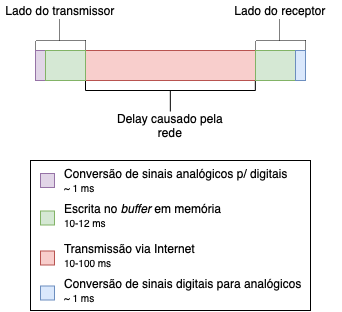
\includegraphics[width=0.5\textwidth]{images/streaming-latency.png}
\caption{Latências de cada fase do processo de \textit{streaming} de áudio pela Internet}
\label{fig:streaming_latencies}
\end{figure}

Aplicações comerciais de videoconferências, como o \textit{Zoom}, \textit{Google Meet} e \textit{FaceTime} também  possuem sensibilidade de tempo para manter conversas compreensíveis - a \textit{Cisco} define a latência máxima aceitável de uma implementação \textit{VoIP} em até 150 ms \cite{cisco}. Este limite pode ser alcançado por conexões de velocidades medianas, mesmo considerando fatores como processamento de áudio, distância entre os participantes e infraestruturas de rede compartilhadas. No entanto, para a prática colaborativa musical, onde tolerância máxima é bastante restrita - variando entre 10 ms e 55 ms \cite{mcphearson} - mostra-se inviável. Em ambientes de alta latência, músicos tendem a perceber incômodos e mudam a forma sobre como performam para adaptarem-se. \cite{carot_low_latency}.

A tolerância de atraso para a performance musical, portanto, é o maior desafio na implementação de ambientes colaborativos musicais \textit{online}. Afinal, mesmo considerando a velocidade da luz no vácuo - aproximadamente 300 km/ms \cite{speed_of_light} - a menor distância possível para obter uma latência ótima de 10 ms é de aproximadamente 3.000 km - um pouco mais que a distância entre Recife, PE e Porto Alegre, RS\footnote{Distância calculada utilizando o Google Maps. ©2021 Google}.

Dessa forma, métodos para redução da latência entre os participantes - ou a sensação de sua existência - possuem suma relevância para músicos. Em contextos onde a presença física dos participantes não é possível de se obter, como o recomendado pelo distanciamento social como método de prevenção de contaminação na Pandemia de COVID-19, a colaboração \textit{online} é o único meio onde músicos conseguem tocar em conjunto.
\section{Estado da arte}

% quais são as soluções atuais para o problema? Como elas atendem os "critérios de avaliaçao"? O que pode serve de inspiração para sua solução?
% no caso de problema/solução original, faz um estado da arte de delimitação do escopo (eu conheo o que existe o suficiente para dizer que ninguém)

Para resolver o problema da latência em ambientes musicais, identificamos duas abordagens principais: (1) otimizações na camada de transporte da Internet e (2) criação de ambientes assíncronos, onde os músicos não performam em tempo real uns com os outros.

\subsection{Otimizações na camada de transporte}

Esta abordagem procura atacar o problema de forma mais linear, implementando melhorias na conexão pela Internet entre os participantes ou utilizando infraestruturas de rede específicas.

\textit{LoLa} (\textit{LOw LAtency audio visual streaming system}) \cite{lola}, um sistema de \textit{streaming} audio visual desenvolvido pelo \textit{Conservatorio di Musica G. Tartini}, consegue atingir conexões de baixa latência, utilizando infraestruturas de rede dedicadas. Foi usado em diversas apresentações de até 3.500 km de distância entre os músicos entre os anos de 2010 e 2013 \cite{lola_streaming}. No entanto, deixa muito claro que sua solução não é necessariamente acessível, sendo recomendado no mínimo 1 Gigabit por segundo de banda em todas as pontas. De acordo com estudo realizado pela Viavi Solutions em 2019, apenas 5\% da população mundial possui conexões tão rápidas \cite{1gbps}, e a média de velocidade mundial é de apenas 97.52 Megabits por segundo, pelos dados apresentados pelo Speedtest Global Index \cite{speed_test}. Portanto, para o público em geral, não é uma solução de fácil acesso.

\textit{SoundJack} \cite{soundjack}, por outro lado, utiliza-se de alguns métodos que o torna mais acessíveis para o usuário comum. Ele consegue atingir velocidades mais rápidas que aplicações comerciais como \textit{Zoom}, \textit{Teams} e \textit{FaceTime} por dois fatores: (1) conecta usuários diretamente através de P2P (\textit{peer-to-peer}), ao contrário das soluções citadas, que transportam dados entre servidores centrais e (2) não otimiza a qualidade o áudio/vídeo automaticamente, deixando como responsabilidade do usuário; caso prefiram, os músicos podem optar por conexões de menores latências assumindo o custo de obter piores qualidades de áudio. Nas configurações recomendadas, infraestruturas comerciais comuns residenciais são suportadas via Ethernet. Entretanto, \textit{SoundJack} requer um poder computacional relativamente alto para atingir baixas latências - recomenda no mínimo processadores i7 Quad Core, custando cerca de R\$2456,90 \footnote{Preço encontrado na Amazon Brasil em 04/04/2021.}, também oferecendo um dispositivo próprio dedicado à aplicação, vendendo por €226,05 \footnote{Preço encontrado na Symonics em 04/04/2021.}.

A aplicação comercial \textit{JamKazam} \cite{jamkazam} também baseia-se em entrega síncrona dos pacotes de áudio para construir um ambiente musical colaborativo \textit{online}. De acordo com seus os resultados apresentados, é possível performar em conjunto com baixas latências onde os músicos estejam em um mesmo estado, numa distância média de 490 km \cite{jamkazam_video}. Porém, entre maiores distâncias ou infraestruturas não baseadas em fibras, a latência excelente recomendada pela aplicação de 30 ms \cite{jamkazam_latencies} é difícil de ser obtida.

TODO: JackTrip

\subsection{Criação de ambientes assíncronos}

Uma solução que possibilita a percepção de baixa latência é abdicar do requisito de entregar uma experiência em tempo real. Caso seja possível atrasar a entrega dos pacotes de forma não perceptível e, portanto, aumentando a janela mínima de espera, não é necessário possuir baixas latências.

A aplicação \textit{jammr} \cite{jammr} aproveita o conceito de progressão de acordes da teoria musical a seu favor. A cada \textit{loop}, os participantes ouvem o que foi tocado na última iteração pelos seus colegas. Dessa forma, por não ser necessário manter as performances em sincronia, há uma tolerância muito maior às latências causadas tanto pela camada de transporte como as causadas pelos processamentos de áudio locais. No entanto, tal solução necessita que os músicos toquem a mesma progressão em \textit{loop}, funcionando bem para improvisações simples (\textit{jam sessions}); porém, para músicas mais complexas, o sistema não é ideal.

\section{Predição no lado do cliente}
\label{sec:client_side_prediction}

No contexto de videogames, alguns gêneros possuem problemas semelhantes aos que os ambientes musicais enfrentam. Aqueles que utilizam reações como uma das mecânicas de \textit{gameplay}, como luta e FPS (\textit{first-person shooter}), para implementar funcionalidades \textit{online}, necessitam que haja pouco atraso entre os \textit{inputs} dos jogadores.

Há duas vertentes de implementação de jogabilidade \textit{online} em videogames - (1) \textit{Delay-based} (``baseado em atraso'')\cite{rollback} e (2) \textit{Client-side prediction} (``Predição no lado do cliente'', popularmente conhecido como \textit{Rollback Netcode})\cite{client-side-prediction}.

\subsection{\textit{Delay-based}}

Nessa abordagem, todos os \textit{inputs} dos transmissores são esperados antes que as ações correspondentes possam ser executadas \cite{rollback}. Essa implementação é trivial e garante a corretude dos dados transmitidos; no entanto, para conexões de alta latência, nas quais o tempo de transmissão via Internet é maior que a latência de ação local, os jogadores experienciam uma sensação de ``lentidão''.

Esse limite máximo de latência de transmissão varia a cada jogo. Para oferecerem uma experiência fluida, de acordo com o tempo de reação à estímulos visuais, é esperado que não haja mais que 100 ms de atraso entre as ações dos jogadores \cite{pubnub}. Esse limite, no entanto, é apenas uma estimativa - idealmente, a melhor implementação deve garantir que não haja diferença entre jogar \textit{online} ou localmente. Esse limite dependerá de especificações de cada jogo, como FPS (\textit{frame-per-second}), a latência natural causada pelo dispositivo de controle (\textit{input delay}) e suas mecânicas de jogabilidade. Desenvolvedores também podem adicionar um atraso artificial, objetivando aumentar a tolerância de tempo causado pela transmissão dos pacotes via Internet.

No contexto de ambientes musicais \textit{online}, podemos comparar esse método com as soluções síncronas citadas na \secref{sec:delay-based-audio-solutions}. Nesses casos, assim como presente no contexto de videogames, essa técnica é muito sensível à latência causada pela transmissão de pacotes via Internet entre os participantes. As soluções citadas, portanto, focam em reduzir o tempo total de transmissão, mas são limitadas por fatores externos, exigindo bandas de alta velocidade e/ou proximidade geográfica.

\subsection{\textit{Client-side prediction}}

A implementação do \textit{Client-side prediction} \footnote{Tradução da imagem criada por GerardSN, CC BY-SA 4.0. Disponível em https://commons.wikimedia.org/w/index.php?curid=97477279.} (\figref{fig:rollback_diagram}), por outro lado, aumenta a tolerância da espera dos pacotes propondo a previsão dos \textit{inputs} dos jogadores antes que cheguem via Internet utilizando dados já recebidos anteriormente. Caso as previsões sejam incorretas, o estado de jogo no momento em que a previsão foi realizado é retornado, portanto, o nome popular ``\textit{rollback}'' (reversão) \cite{rollback}.

\begin{figure}[htbp]
\centering
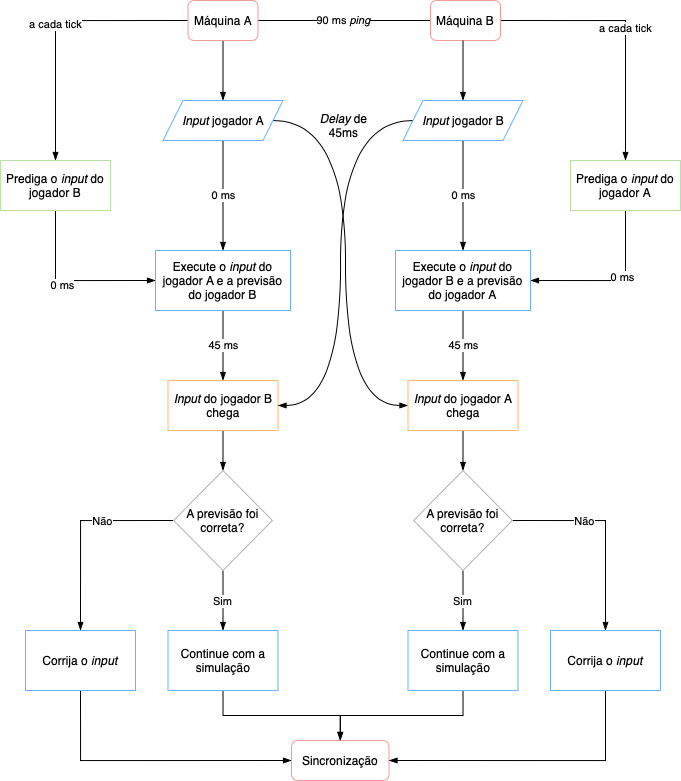
\includegraphics[width=1\textwidth]{images/rollback.png}
\caption{Diagrama demonstrando o processo de execução e sincronização dos \textit{inputs} de dois jogadores (com \textit{ping} de 90 ms entre eles) em um jogo \textit{online} utilizando \textit{client-side prediction} em um modelo \textit{peer-to-peer}.}
\label{fig:rollback_diagram}
\end{figure}

A necessidade da implementação do \textit{client-side prediction} surge em 1996, em um contexto onde a maioria dos usuários de Internet possuíam conexões discadas com banda entre 28 Kb/s e 34 Kb/s \cite{broadband}. \textit{Duke Nukem 3D}, um jogo do gênero FPS (\textit{first-person shooter}, ``tiro em primeira pessoa''), foi pioneiro na utilização desse algoritmo para prover sincronia entre os jogadores \textit{online} \cite{duke_nukem}, que podem possuir diferentes velocidades de Internet ou estarem distantes entre si. Os \textit{inputs} dos jogadores remotos eram previstos no lado do cliente e enviados a um servidor central, que comparava os \textit{inputs} corretos e enviava as correções necessárias.

O modelo de previsão, isto é, o algoritmo utilizado para prever os \textit{inputs} dos jogadores remotos, pode variar de acordo com as necessidades específicas dos jogos. O modelo proposto por Bernier, utilizado no jogo \textit{Half-Life}, apenas repete os últimos \textit{inputs} reconhecidos pelo servidor \cite{client-side-prediction}. Esse modelo assume que os \textit{inputs} tendem a se repetir com frequência a cada \textit{frame}, portanto, apenas repeti-los e corrigir aqueles que não se enquadram funciona bem para a maioria dos casos.

A utilização de \textit{client-side prediction} expande-se para diferentes gêneros, como o de luta, e sua adoção é vista positivamente pelos jogadores \cite{rollback_success}. Por não necessitar esperar os \textit{inputs} dos adversários para execução do jogador localmente, a sensação de fluidez é mais aparente do que as implementações baseadas em atraso.

No entanto, por não garantir a corretude dos \textit{inputs} imediatamente após a previsão, é necessário haver a correção do estado do jogo em caso de erro da previsão. Essa correção pode causar, por exemplo, que um jogador perceba que seu adversário está em uma determinada posição no espaço e, em outro momento, mudar de lugar instantaneamente, causando uma sensação de ``teletransporte''. Fatores como \textit{FPS} (\textit{frames per second}, ``quadros renderizados por segundo'') e a latência entre os jogadores, que não são valores constantes, desafiam os desenvolvedores a manter a sincronia entre todos os clientes \cite{client-side-prediction}.
\chapter{Proposta de solução}

No contexto de videogames que utilizam reações visuais/auditivas como mecânica essencial de jogabilidade possuem alta sensibilidade à latência de \textit{inputs}. Como forma de mitigar esse problema, a técnica de previsão no lado do cliente, como descrito na \secref{sec:client_side_prediction}, é implementada em diversos \textit{games} e é muito bem vista pelos jogadores.

Paralelamente, ao observar ambientes musicais \textit{online}, percebe-se o mesmo requisito de baixa latência para manter a fluidez dos participantes, como descrito na \secref{sec:problem}. Portanto, questiona-se: é possível aplicar técnicas de predição no lado do cliente nesse contexto, de forma a permitir sessões artísticas satisfatórias entre os artistas?

Evidentemente, apesar de compartilharem a baixa tolerância a latência, a natureza dos problemas são significativamente divergentes. A mera implementação de previsão no lado do cliente no contexto musical implica em dois grandes problemas: (1) a impossibilidade de retornar ao último momento da música em caso de erro na previsão e; (2) a enorme dimensionalidade da representação digital de áudio.

A aplicação de previsão no lado do cliente, quando aplicado a videogames, baseia-se no fato que os eventuais retornos ao estado anterior à previsão em caso de erros não são suficientemente prejudiciais à experiência do jogador. No contexto de música, no entanto, devido sua natureza contínua na linha do tempo, o conceito de "estados" não pode ser replicado e, portanto, não faz sentido retornarmos a um momento anterior.
 
Ademais, a quantidade de \textit{inputs} produzidos pelos jogadores é ínfima quando comparada a representação de áudio digital. Estima-se que os jogadores profissionais de \textit{Super Smash Bros. Melee} mais técnicos produzem em média 6 \textit{inputs} por segundo \cite{melee_inputs_per_second}, variando de acordo com o momento do jogo. Por outro lado, uma transmissão de áudio com \textit{sample rate} de 44,1 Khz produz consistentemente, por definição, 44.100 diferentes valores no mesmo espaço de tempo \cite{jukebox_dimension}. O modelo preditivo proposto por Bernier \cite{client-side-prediction} replica os últimos \textit{inputs} reconhecidos pelo servidor; se aplicássemos o mesmo conceito em música, efetivamente estaríamos "atrasando" os \textit{inputs} musicais.

Portanto, a acurácia do modelo preditivo em ambientes musicais é de suma importância, uma vez que a "volta no tempo" é impossível. Atingir esse alto nível de acurácia, por sua vez, é um enorme desafio, dada a dimensionalidade da representação de áudio digital. Naturalmente, o tempo total gasto na geração da previsão não pode exceder o tempo da janela prevista - caso ocorra, retornaremos ao mesmo problema enfrentado pelas soluções síncronas apresentadas na sessão \secref{sec:delay-based-audio-solutions}. 

Propomos, então, uma variação da implementação de Bernier \cite{client-side-prediction} de previsão no lado do cliente, para sua aplicação no contexto musical (\figref{fig:rollback_music_diagram}). Similarmente à técnica original, janelas de áudios são previstos baseando-se em entradas anteriores. Entretanto, nenhuma correção é feita, mantendo a linearidade da música.

\begin{figure}[htbp]
\centering
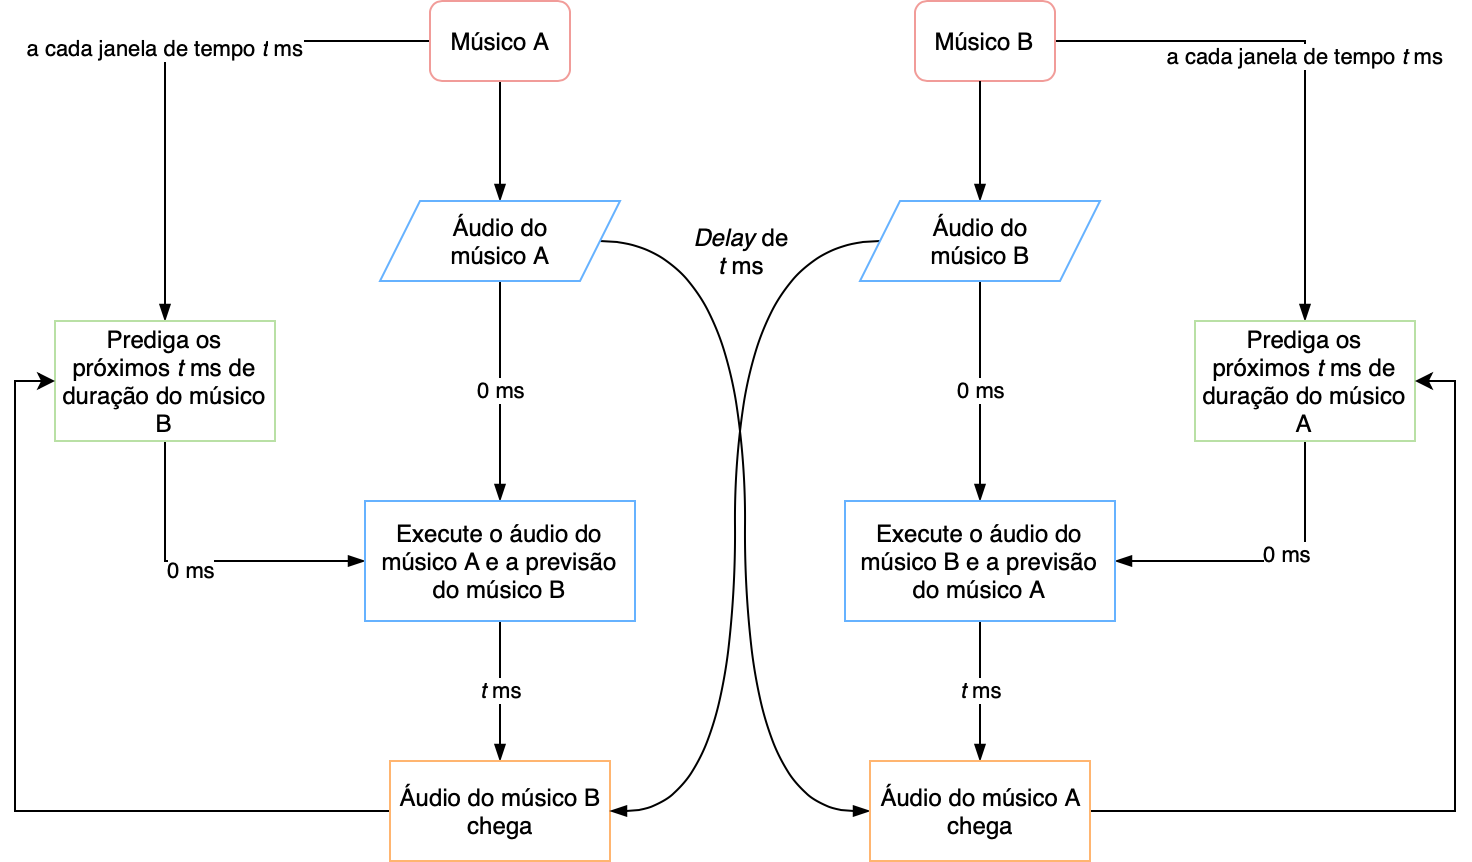
\includegraphics[width=1\textwidth]{images/rollback-music.png}
\caption{Diagrama demonstrando a adaptação do algoritmo de previsão no lado do cliente aplicado para \textit{streaming} colaborativo de música \textit{online}. Na imagem, "X" representa a duração da janela de previsão, medido em milissegundos.}
\label{fig:rollback_music_diagram}
\end{figure}

Em Bernier, a janela de tempo de cada conjunto de previsões é definida de acordo com o FPS e a velocidade de conexão entre os participantes. Na adaptação musical, além do tempo de ida e volta dos pacotes entre os participantes (\textit{ping}), propomos a utilização de outros parâmetros para a decisão dessa janela, como o BPM (batimentos da música) ou valores arbitrários. A escolha dessa janela é fundamental - durações muito longas possuem muita informação, porém, são mais difíceis de processar; e o inverso ocorre para janelas muito curtas.

Propomos, portanto, dois modelos preditivos para música, dividido em dois ciclos de pesquisa. No (CITAR CAPITULO), utilizamos a arquitetura de aprendizagem de máquina em camadas LSTM (\textit{Long short-term memory)} \cite{lstm} para gerar sequências de sinais digitais. Já em (CITAR CAPITULO), no segundo ciclo, usamos o algoritmo DTW (\textit{Dynamic Time Warping}) \cite{dtw} para identificar janelas semelhantes em uma base de dados e, a partir dessa informação, reproduzir a próxima janela de áudio, também armazenada na mesma base de dados.


% Ao observar o contexto de videogames, encontramos requisitos de latência similares. Gêneros que utilizam reações como mecânica de jogabilidade, como luta e FPS (\textit{first-person shooter}), para oferecerem aos jogadores uma experiência fluida, necessitam de latências máximas de até 100 ms \cite{pubnub}. O algoritmo mais popular e efetivo para solucionar esse problema, \textit{client-side prediction} \cite{client-side-prediction}, baseia-se em prever os próximos \textit{inputs} imediatos dos jogadores e agindo antes mesmo que os dados de seu oponente sejam transmitidos; desta forma, removendo a necessidade inicial de espera. Uma vez que os \textit{inputs} são recebidos, estes são comparados com a previsão realizada e, caso sejam incongruentes entre si, o jogo é retornado ao estado anterior do momento da previsão inicial.

% Por possuir requisitos semelhantes de baixa latência, a mesma implementação baseada em previsões tem o potencial de resolver o problema descrito anteriormente para ambientes musicais colaborativos \textit{online}. Caso seja possível prever os próximos sinais digitais produzidos pelos artistas remotos, não haveria necessidade de espera e, portanto, a latência de rede tornaria-se irrelevante.

% Evidentemente, as diferenças entre os contextos de \textit{videogames} e práticas musicais não são negligenciáveis. Ao contrário dos jogos, por apresentar uma linearidade no tempo, não é possível retornar ao último momento da música anterior à previsão imediata sem atrapalhar a performance dos artistas. Além disso, a natureza discreta dos \textit{inputs} dos \textit{videogames} e a quantidade bruta de dados produzida é ínfima em comparação à áudios digitais - estima-se que os jogadores profissionais de \textit{Super Smash Bros. Melee} mais técnicos produzem em média 6 \textit{inputs} por segundo \cite{melee_inputs_per_second}; uma transmissão de áudio com \textit{sample rate} de 44,1 khz produz, por definição, 44.100 diferentes valores no mesmo espaço de tempo \cite{jukebox_dimension}. Portanto, a aplicação do algoritmo de \textit{client-side prediction} para transmissão de música \textit{online} não é trivial, e a necessidade que o modelo preditivo seja o mais acurado possível é ainda mais importante.
\section{Adaptação do \textit{client-side prediction} no contexto musical \textit{online}}

Propomos, então, uma variação da implementação de Bernier \cite{client-side-prediction} de previsão no lado do cliente, para sua aplicação no contexto musical (\figref{fig:rollback_music_diagram}). Similarmente à técnica original, janelas de áudios são previstos baseando-se em entradas anteriores. Entretanto, nenhuma correção é realizada em casos de erro, mantendo a linearidade da música.

\begin{figure}[htbp]
\centering
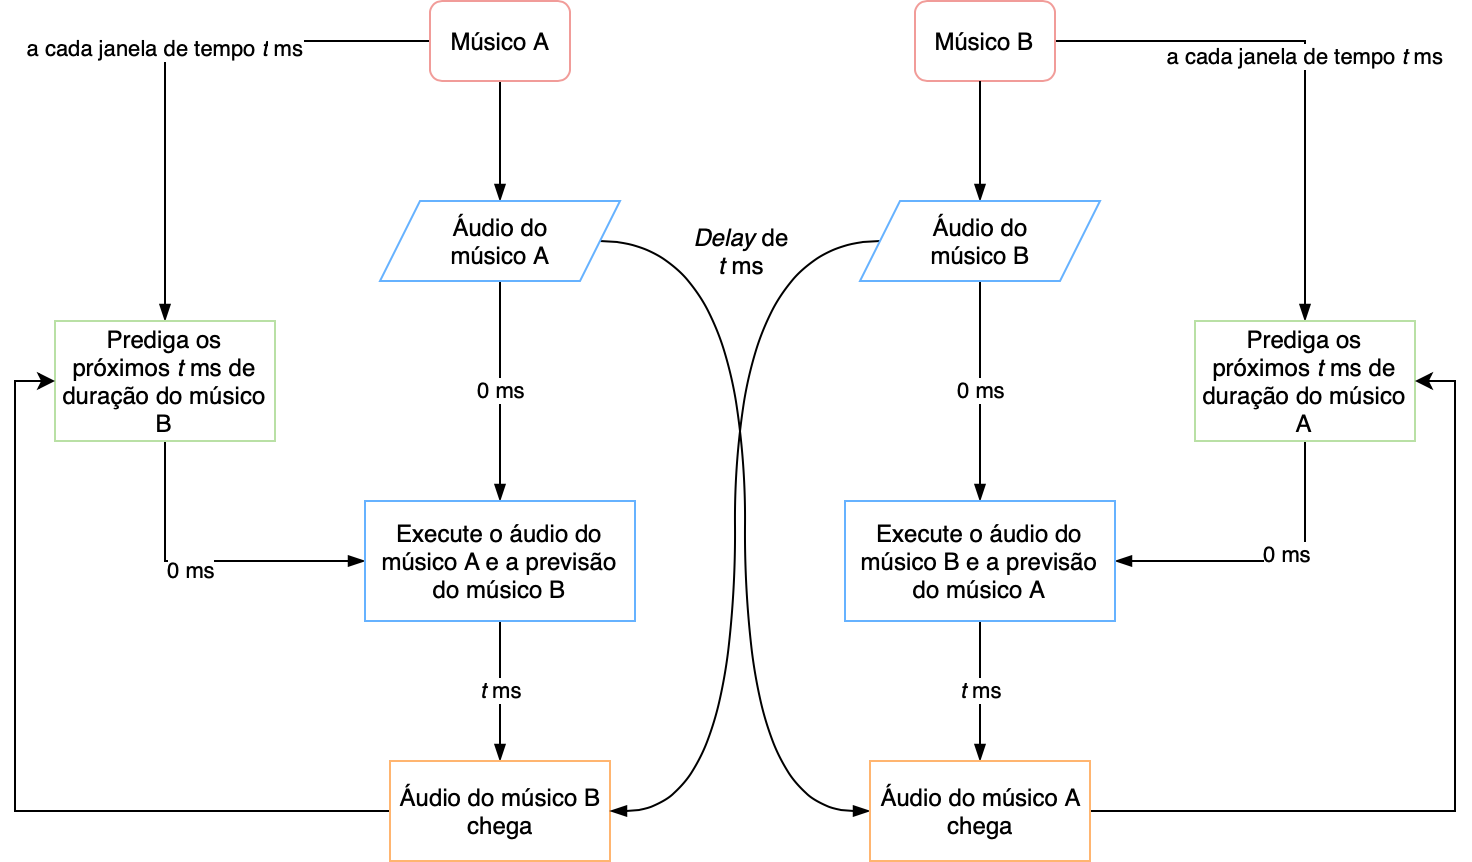
\includegraphics[width=1\textwidth]{images/rollback-music.png}
\caption{Diagrama demonstrando a adaptação do algoritmo de previsão no lado do cliente aplicado para \textit{streaming} colaborativo de música \textit{online}. Na imagem, $t$ representa a duração da janela de previsão, medido em milissegundos.}
\label{fig:rollback_music_diagram}
\end{figure}

Em Bernier, a janela de tempo de cada conjunto de previsões é definida de acordo com o FPS e a velocidade de conexão entre os participantes. Para adaptação musical, além do tempo de ida e volta dos pacotes entre os participantes (\textit{ping}), propomos a utilização de outros parâmetros para a decisão dessa janela, como o BPM (batimentos por minuto) da música tocada ou outros valores arbitrários. A escolha dessa janela é fundamental - durações muito longas possuem muita informação, porém, são mais difíceis de processar; e o inverso ocorre para janelas muito curtas.

Propomos, portanto, dois modelos preditivos para música, explorados em dois ciclos de pesquisa. No \chapref{chap:lstm}, o primeiro ciclo, utilizamos a arquitetura de aprendizagem de máquina em camadas LSTM (\textit{Long short-term memory)} \cite{lstm} para gerar sequências de sinais digitais, baseadas nas entradas anteriores. Já no \chapref{chap:dtw}, no segundo ciclo, usamos o algoritmo DTW (\textit{Dynamic Time Warping}) \cite{dtw} para identificar janelas semelhantes em uma base de dados e, a partir dessa informação, reproduzir a próxima janela de áudio, também armazenada na mesma base de dados.

\section{Métricas de sucesso dos modelos preditivos}
\label{sec:success_metrics}

Como mencionado, existem alguns requisitos que os modelos preditivos propostos precisam cumprir para serem considerados bem sucedidos. Em cada ciclo, diferentes metodologias foram utilizadas para demonstrar essas métricas.

\subsection{Corretude das previsões}
\label{subsec:prediction_correctness}

Devido à característica de linearidade de tempo que a música possui, não é possível ``retornar'' a um estado passado da música. Dessa forma, é importante que os modelos sejam os mais acurados possíveis.

Dada a natureza da predição, não é esperado que as sequências geradas sejam integralmente fidedignas às sequências reais. No entanto, isso não é um requisito para produzir resultados positivos, sendo realmente importante que os áudios previstos tenham a mesma ``intenção'' que a reprodução original.

Dessa forma, o critério de sucesso dessa métrica é, para as sequências previstas, que seja imperceptível, em tempo real, que haja diferenças entre as sequências originais; de forma que um músico, ao ouvir ambas as sequências, reagiria musicalmente da mesma maneira ou de maneira similar.

Note que, por se tratar de um critério abstrato, quantificar essa métrica pode não representar bem o seu sucesso. Em cada um dos ciclos, utilizamos diferentes metodologias (demonstrados em \secref{sec:lstm_metodology} e \secref{sec:dtw_metodology}) para medi-la, visando sempre satisfazer o critério estabelecido.

\subsection{Tempo de geração de previsões}
\label{subsec:time_metric}

Supondo que \textit{t} é o tempo escolhido das janelas de previsão de áudio e \textit{p} é o tempo levado para gerar essas previsões, é imprescindível para o sucesso dos modelos preditivos que $t \leq p $. Caso contrário, o tempo excedente de processamento cria um \textit{delay} entre o que está sendo executado pelo músico remoto e o que está sendo reproduzido localmente e, consequentemente, causando dessincronia entre os músicos.

Ao contrário do critério de corretude na \secref{subsec:prediction_correctness}, essa métrica consegue ser medida precisamente. Será considerado bem sucedida o modelo preditivo que produzir sequências em um tempo menor que a duração do áudio gerado.

\chapter{Ciclo 1: Geração de novas sequências com LSTM}
\label{chap:lstm}
\section{Proposta de solução}

% • Princípios, inspirações, ideias gerais
% • Descrição detalhada da solução
% • implementação (arquitetura, tecnologias, etc.)

TODO: explicar proposta de solução do LSTM

- Explicar sobre a escolha do tamanho da janela
\section{Avaliação}

% • Metodologia
% • Resultados obtidos
% • Análise: discussão dos resultados

TODO: mostrar resultados.

- Imagem dos sinais sobrepondo-se
- Acabou repetindo os dados de entrada
\chapter{Ciclo 2: Indexação com DTW}

TODO: explicar a ideia do DTW vinda a partir dos resultados do primeiro ciclo
\section{Proposta de solução}

% • Princípios, inspirações, ideias gerais
% • Descrição detalhada da solução
% • implementação (arquitetura, tecnologias, etc.)

TODO: explicar proposta de solução com DTW

- imagem do encontro dos áudios
- relembrar sobre o dilema da escolha de duração da janela
\section{Avaliação}

% • Metodologia
% • Resultados obtidos
% • Análise: discussão dos resultados

TODO: mostrar tabela dos resultados

- Explicar o que acontece sonoramente na transição
\chapter{Conclusões}
\label{chap:conclusion}

De acordo com nosso experimentos, o modelo preditivo gerador de novas sequências com LSTM não teve bom desempenho em nenhuma das duas métricas de sucesso estabelecidas na \secref{sec:success_metrics}. Por repetir os dados de entrada, caso utilizássemos esse modelo em uma aplicação real, estaríamos apenas atrasando o áudio transmitido e replicando o problemas que as soluções síncronas enfrentam hoje.

Além disso, devido ao alto tempo necessário para realizar a predição, tal solução mostrou-se inviável da forma que foi implementada. Para atingir tempos menores, seria necessário mais poder computacional, tornando essa solução inacessível para a população em geral.

Portanto, de acordo com nossos experimentos, o modelo gerador com LSTM não se mostrou promissor para ser utilizado em uma adaptação do \textit{client-side prediction} para ambientes musicais. Porém, melhorias podem ser estudadas que viabilizem seu uso, exploradas na \secref{sec:later_work}.

Entretanto, no segundo ciclo, o modelo indexador e identificador mostrou-se bastante promissor em nossos experimentos. Apesar de possuir uma base da dados pequena, a taxa de acerto das previsões foi consideravelmente alta, de forma a trazer a sensação de fluidez nos momentos de acerto na previsão. Se relacionarmos com o \textit{client-side prediction}, que corrige os \textit{inputs} dos jogadores sempre que há um erro, os erros nas previsões realizadas podem ser aceitáveis.

Ademais, o tempo necessário para apontar as predições foi bastante baixo, deixando espaço suficiente para que máquinas menos potentes do que a utilizada nos experimentos possam usufruir dessa abordagem.

Porém, não podemos afirmar com certeza suficiente que o modelo indexador pode ser utilizado em aplicações reais. A base de dados utilizada foi propositalmente reduzida para testar a validade do modelo, possibilitando altas taxas de acertos na identificação e alta eficiência. Além disso, as janelas de áudio escolhidas são consideravelmente altas, o que impede seu uso em improvisações musicais.

Entretanto, o modelo indexador com DTW mostrou-se bastante promissor para uso na adaptação do \textit{client-side prediction} para ambientes musicais, principalmente para músicos de base, que não tendem a improvisar em suas performances.



%%
%% Parte pós-textual
%%
\backmatter

% Apêndices
% Comente se não houver apêndices
\appendix

% É aconselhável criar cada apêndice em um arquivo à parte, digamos
% "apendice1.tex", "apendice.tex", ... "apendiceM.tex" e depois
% incluí-los com:
% \include{apendice1}
% \include{apendice2}
% ...
% \include{apendiceM}


% Bibliografia
% É aconselhável utilizar o BibTeX a partir de um arquivo, digamos "biblio.bib".
% Para ajuda na criação do arquivo .bib e utilização do BibTeX, recorra ao
% BibTeXpress em www.cin.ufpe.br/~paguso/bibtexpress
\nocite{*}
\bibliographystyle{ieeetr}
\bibliography{references}

% Cólofon
% Inclui uma pequena nota com referência à UFPEThesis
% Comente para omitir
% \colophon

%% Fim do documento
\end{document}
